
%
%  $Description: Author guidelines and sample document in LaTeX 2.09$ 
%
%  $Author: ienne $
%  $Date: 1995/09/15 15:20:59 $
%  $Revision: 1.4 $
%
% !TEX encoding = UTF-8 Unicode

\documentclass[times, 10pt,twocolumn]{article} 
\usepackage{latex8}
\usepackage{times}
\usepackage[utf8x]{inputenc}
\usepackage {graphicx}


%\documentstyle[times,art10,twocolumn,latex8]{article}

%------------------------------------------------------------------------- 
% take the % away on next line to produce the final camera-ready version 
\pagestyle{empty}

%------------------------------------------------------------------------- 
\begin{document}

\title{\LaTeX\ Author Guidelines 
       for {\boldmath $8.5 \times 11$-Inch} Proceedings Manuscripts}

\author{Bernardo Simões\\ Afonso Oliveira\\ Rui Francisco\\
Instituto Superior Técnico\\Plataformas para Aplicações Distribuídas da Internet\\
% For a paper whose authors are all at the same institution, 
% omit the following lines up until the closing ``}''.
% Additional authors and addresses can be added with ``\and'', 
% just like the second author.
}

\maketitle
\thispagestyle{empty}

\begin{abstract}
No projecto de PADI (Plataformas para Aplicações Distribuídas na Internet), foi-nos pedido para projectar e implementar uma PADITable, um sistema distribuído que gere em memória volátil conjuntos de chave-valor que suportam as duas operações fundamentais \emph{get} e \emph{put} de forma atómica.
Este documento contem a descrição dos protocolos implementados para a nossa solução deste sistema, onde discutimos formas de processamento de transacções atómicas, topologia da rede e gestão dos servidores, clientes e uma directoria central. Seguidas de uma avaliação das mesmas referindo vantagens e desvantagens de cada implementação e são apresentados resultados.
\end{abstract}



%------------------------------------------------------------------------- 
\Section{Introdução}

Este artigo permite descrever a solução para a implementação da \emph{PADITable}, um sistema distribuído para gerir o armazenamento volátil de conjuntos chave-valor. Este sistema é constituído por 4 tipos de nós: uma directoria central (referida em frente como o nó CD (\emph{Central Directory}), um conjunto de servidores e um conjunto de clientes que são controlados por um \emph{puppet master}. Os conjuntos chave-valor estão armazenados nos servidores que são operados pelos clientes usando operações de \emph{put} e \emph{get}. A directoria central tem a informação dos clientes e servidores ligados à rede e o \emph{puppet master} é responsável por controlar os clientes a fim de testar e fazer \emph{debug} do sistema.

Como todos os sistemas distribuídos é necessário saber onde colocar determinada informação. Como tal é necessário um algoritmo para dividir diferentes chaves pelos servidores existentes de maneira a no futuro se saber melhor onde se encontra cada chave. A este problema segue-se o problema de que os servidores do sistema podem iniciar-se em alturas diferentes, o que faz com que a distribuição anterior de chaves fique desactualizada. Será então necessário mover a localização de algumas chaves a fim de tornar o sistema mais e melhor distribuído.

Quando um cliente precisar de executar operações de \emph{put} e \emph{get} irá necessitar de saber a localização dos servidores com as chaves a que quer aceder ou então será necessário um sistema para reencaminhar os pedidos para o servidor certo. A solução para este problema deverá usar o menor número de comunicações possível a fim de ser uma solução optimizada.

Uma vez que o cliente saiba a localização dos servidores que necessita aceder, ele terá de assegurar que uma transacção completa se executa de maneira sequencial de maneira a evitar estados inconsistentes.

A fim de se aumentar a disponibilidade do sistema e aumentar a capacidade de acesso a uma chave o sistema irá ser replicado. Onde e como replicar a informação é um factor que deve ser tomado em conta e que terá impacto no desempenho do sistema. Esta replicação deverá tornar o sistema acessível em caso de falha de qualquer servidor. A informação replicada deverá estar sempre consistente de maneira a evitar que sejam lidos valores desactualizados.

O sistema deverá estar preparado para que em cada chave sejam guardados vários valores, cada um associado a uma marca temporal. O sistema guarda assim um historial de valores antigos. Esta situação pode ser usada para diminuir o número de operações apenas de leitura que falham.

Na secção \ref{secSol} irão ser identificadas e descritas as soluções para os requisitos do sistema e os problemas que estes levantam. De seguida na secção \ref{secAdv} irão ser descritas as vantagens das soluções optadas. Nesta secção serão também apresentados resultados de \emph{benchmarks} ao sistema implementado, descrevendo o impacto das decisões tomadas nos valores obtidos.

\begin{figure}[h]
\centering
	 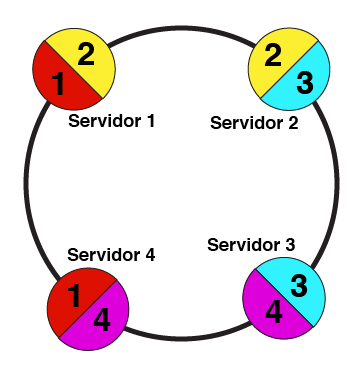
\includegraphics[width=0.35\textwidth]{replication}
   \caption{Replicação da Informação.}
\end{figure}
%------------------------------------------------------------------------- 
\Section{Solução}

Please read the following carefully.

%------------------------------------------------------------------------- 
\SubSection{Algoritmos de Colocação de Dados}

%------------------------------------------------------------------------- 
\SubSection{Encaminhamento}

%------------------------------------------------------------------------- 
\SubSection{Protocolo de Transacções e Consistência de Réplicas}

\begin{figure}[h]
\centering
	 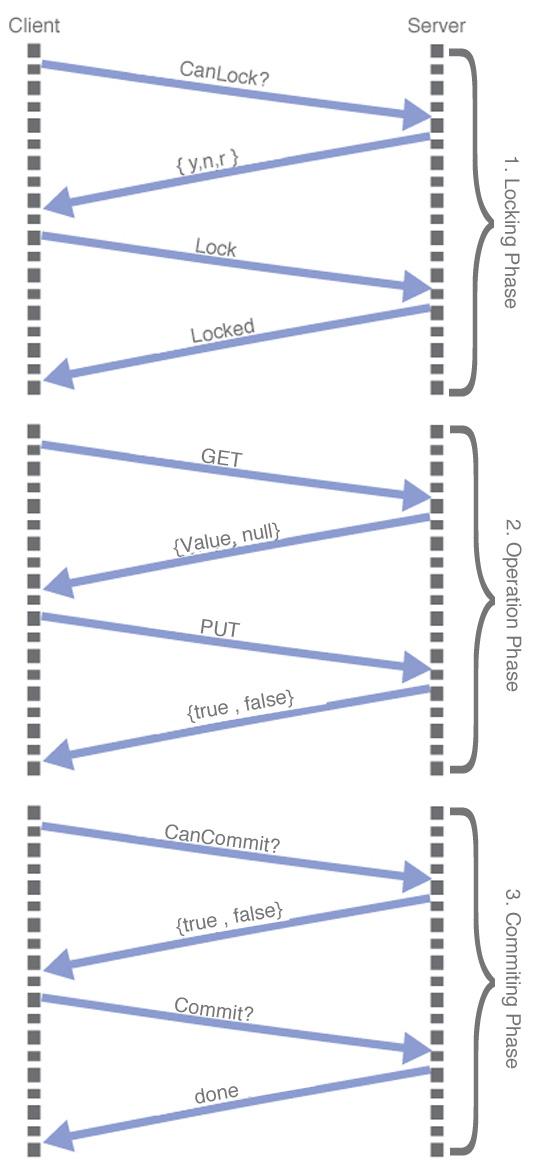
\includegraphics[width=0.35\textwidth]{TransactionDiagram}
   \caption{Example of caption.}
\end{figure}

%------------------------------------------------------------------------ 
\SubSection{Falhas do Servidor}

%------------------------------------------------------------------------- 
\SubSection{Multi-Vers√£o}

%------------------------------------------------------------------------- 

\Section{Vantagens e Desvantagens da Solução}
\Subsection{Colocação e Localização da Informação}
\Subsection{Vantagens do Protocolo Transaccional}
\Subsection{Vantagens da Consistência das Réplicas}
\Subsection{Vantagens da Multi-Versões}

\Section{Conclus√£o}
\Subsection{Transacções}

%------------------------------------------------------------------------- 
\nocite{ex1,ex2}
\bibliographystyle{latex8}
\bibliography{latex8}

\end{document}

